\documentclass[11pt, a4paper]{article}

% Set up the page
\usepackage{pdflscape}
\usepackage{fullpage}
\usepackage{graphicx}
\usepackage[normalem]{ulem}  % for the dashed underline
\usepackage{rotating}
\usepackage{multicol}

% Set up Tikz Library
\usepackage{tikz}
\usetikzlibrary{shapes.geometric}
\usetikzlibrary{shapes.multipart}
\usetikzlibrary{positioning}
\usetikzlibrary{arrows}
\usetikzlibrary{arrows.meta}
\usetikzlibrary{fit}
\usetikzlibrary{matrix}
\usetikzlibrary{shadows}
\usetikzlibrary{calc}

% Primary key should be underlined
\newcommand{\primarykey}[1]{\underline{#1}}

%%%%% ENTITY %%%%%%

% Entity - Basic rect
\tikzstyle{entity} = [rectangle, draw, thick, black, minimum width=4em, minimum height=2.5em]

% Weak Entity - Double lined rect
\tikzstyle{weak entity} = [entity, double, double distance=2pt]

%%%%% Attribute %%%%%%

% Attribute - Ellipse around attribute
\tikzstyle{attribute} = [ellipse, draw, black, thick, minimum width=5em, minimum height=2em]

% Multi-value attribute - double circled ellipse
\tikzstyle{multi attribute} = [attribute, double, double distance=2pt]

% Derived attribute - Dashed ellipse
\tikzstyle{derived attribute} = [attribute, dashed]

%%%%% Relationship %%%%%%

% Relationship - diamond
\tikzstyle{relationship} = [diamond, draw, black, thick, minimum width=2em, aspect=1, fill=white]

% Weak Entity Relationship - double diamond
\tikzstyle{weak relationship} = [relationship, double, double distance=2pt]

% IS-A relationship - triangle
\tikzstyle{isa} = [isosceles triangle, isosceles triangle apex angle=60, shape border rotate=120, draw, black, thick, minimum size=3em]

%%% Arrow style

\tikzstyle{oneone} = [-{Latex[width=10mm, length=10mm]}, line width=0.2cm]
\tikzstyle{zeroone} = [-{Latex[width=5mm, length=7mm]}]
\tikzstyle{zeromany} = [--]
\tikzstyle{onemany} = [--, line width=0.2cm]


%%% Crow Foot ERD style - PREFIX with ``cf'' %%%


%
% Crow Foot Many
%

\pgfarrowsdeclare{cfmany}{cfmany}
{
  \pgfarrowsleftextend{+-.5\pgflinewidth}%
  \pgfarrowsrightextend{+.5\pgflinewidth}%
}
{
  \pgfutil@tempdima=0.6pt%
  %\advance\pgfutil@tempdima by.25\pgflinewidth%
  \pgfsetdash{}{+0pt}%
  \pgfsetmiterjoin%
  \pgfpathmoveto{\pgfqpoint{0pt}{-9\pgfutil@tempdima}}%
  \pgfpathlineto{\pgfqpoint{-13\pgfutil@tempdima}{0pt}}%
  \pgfpathlineto{\pgfqpoint{0pt}{9\pgfutil@tempdima}}%
  \pgfpathmoveto{\pgfqpoint{0\pgfutil@tempdima}{0\pgfutil@tempdima}}%
  \pgfpathmoveto{\pgfqpoint{-15pt}{-6pt}}% 
  \pgfpathlineto{\pgfqpoint{-15pt}{-6pt}}%  
  \pgfpathlineto{\pgfqpoint{-15pt}{6pt}}% 
  \pgfusepathqstroke%
}

%
% Crow Foot zero-Many
%

\pgfarrowsdeclare{cfomany}{cfomany}
{
  \pgfarrowsleftextend{+-.5\pgflinewidth}%
  \pgfarrowsrightextend{+.5\pgflinewidth}%
}
{
  \pgfutil@tempdima=0.6pt%
  %\advance\pgfutil@tempdima by.25\pgflinewidth%
  \pgfsetdash{}{+0pt}%
  \pgfsetmiterjoin%
  \pgfpathmoveto{\pgfqpoint{0pt}{-9pt\pgfutil@tempdima}}%
  \pgfpathlineto{\pgfqpoint{-13pt\pgfutil@tempdima}{0pt}}%
  \pgfpathlineto{\pgfqpoint{0pt}{9pt\pgfutil@tempdima}}%
  \pgfpathmoveto{\pgfqpoint{0pt\pgfutil@tempdima}{0pt\pgfutil@tempdima}}%  
  \pgfpathmoveto{\pgfqpoint{0pt\pgfutil@tempdima}{0pt\pgfutil@tempdima}}%
  \pgfpathmoveto{\pgfqpoint{-6pt}{-6pt}}% 
    \pgfpathcircle{\pgfpoint{-16.5pt}{0pt}} {3.5pt}
  \pgfusepathqstroke%
}


%
% Crow Foot One
%

\pgfarrowsdeclare{cfone}{cfone}
{
  \pgfarrowsleftextend{+-.5\pgflinewidth}%
  \pgfarrowsrightextend{+.5\pgflinewidth}%
}
{
  \pgfutil@tempdima=0.6pt%
  %\advance\pgfutil@tempdima by.25\pgflinewidth%
  \pgfsetdash{}{+0pt}%
  \pgfsetmiterjoin%
  \pgfpathmoveto{\pgfqpoint{0\pgfutil@tempdima}{0\pgfutil@tempdima}}%
  \pgfpathmoveto{\pgfqpoint{-6pt}{-6pt}}% 
  \pgfpathlineto{\pgfqpoint{-6pt}{-6pt}}%  
  \pgfpathlineto{\pgfqpoint{-6pt}{6pt}}% 
  \pgfpathmoveto{\pgfqpoint{0\pgfutil@tempdima}{0\pgfutil@tempdima}}%
  \pgfpathmoveto{\pgfqpoint{-8pt}{-6pt}}% 
  \pgfpathlineto{\pgfqpoint{-8pt}{-6pt}}%  
  \pgfpathlineto{\pgfqpoint{-8pt}{6pt}}%    
  \pgfusepathqstroke%
}

%
% Crow Foot zero-One
%

\pgfarrowsdeclare{cfoone}{cfoone}
{
  \pgfarrowsleftextend{+-.5\pgflinewidth}%
  \pgfarrowsrightextend{+.5\pgflinewidth}%
}
{
  \pgfutil@tempdima=0.6pt%
  %\advance\pgfutil@tempdima by.25\pgflinewidth%
  \pgfsetdash{}{+0pt}%
  \pgfsetmiterjoin%
  \pgfpathmoveto{\pgfqpoint{0\pgfutil@tempdima}{0\pgfutil@tempdima}}%
  \pgfpathmoveto{\pgfqpoint{-6pt}{-6pt}}% 
  \pgfpathlineto{\pgfqpoint{-6pt}{-6pt}}%  
  \pgfpathlineto{\pgfqpoint{-6pt}{6pt}}% 
  \pgfpathmoveto{\pgfqpoint{0\pgfutil@tempdima}{0\pgfutil@tempdima}}%
    \pgfpathcircle{\pgfpoint{-12.5pt}{0}} {3.5pt}
  \pgfusepathqstroke%
}

\tikzset{
    zig zag to/.style={
        to path={(\tikztostart) -| ($(\tikztostart)!#1!(\tikztotarget)$) |- (\tikztotarget)}
    },
    zig zag to/.default=0.5,
    cfone to cfone/.style={
        cfone-cfone, zig zag to
    },    
    cfone to cfmany/.style={
        cfone-cfmany, zig zag to,
    },
    cfone to cfomany/.style={
        cfone-cfomany, zig zag to
    },      
    cfmany to cfone/.style={
        cfmany-cfone, zig zag to
    },
    cfmany to cfmany/.style={
        cfmany-cfmany, zig zag to
    },
    cfonemany/.style={
        cfmany-, zig zag to
    },
    cf0many/.style={
        cfomany-, zig zag to
    },
    cfoneone/.style={
        cfone-, zig zag to
    },
    cf0one/.style={
        cfoone-, zig zag to
    }
}
\def\property#1{\node[name=\entityname-#1, every property/.try]{#1};}
\def\properties{\begingroup\catcode`\_=11\relax\processproperties}
\def\processproperties#1{\endgroup%
    \def\propertycode{}%
    \foreach \p in {#1}{%
        \expandafter\expandafter\expandafter\gdef\expandafter\expandafter\expandafter\propertycode%
            \expandafter\expandafter\expandafter{\expandafter\propertycode\expandafter\property\expandafter{\p}\\}%
    }%
    \propertycode%
}

\begin{document}
\begin{landscape}
    \thispagestyle{empty}
    \resizebox{1.3\textwidth}{!}{%
        \begin{center}
          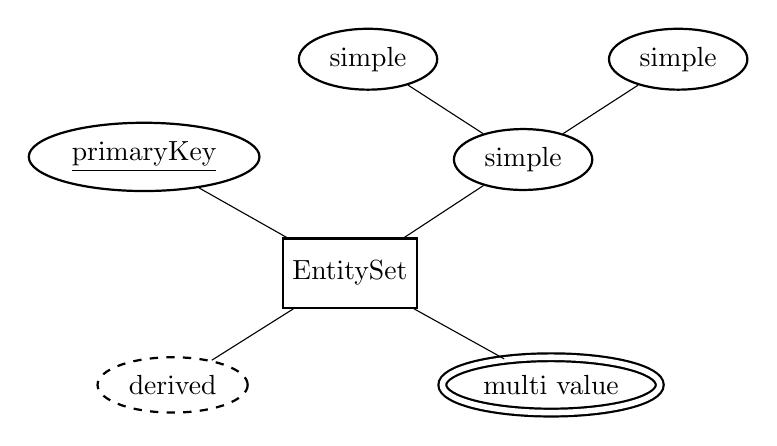
\begin{tikzpicture}
            \node[entity] (entityname) {EntitySet};
            \node[attribute] (primarykeyexample) [above left = 1cm of entityname] {\primarykey{primaryKey}} edge (entityname);
            \node[attribute] (simpleattr) [above right = 1cm of entityname] {simple} edge (entityname);
            \node[attribute] (simpletwo) [above right = 1cm of simpleattr] {simple} edge (simpleattr);
            \node[attribute] (simplethree) [above left = 1cm of simpleattr] {simple} edge (simpleattr);
            \node[derived attribute] (simplederived) [below left = 1cm of entityname] {derived} edge (entityname);
            \node[multi attribute] (multiattr) [below right = 1cm of entityname] {multi value} edge (entityname);
          \end{tikzpicture}
        \end{center}
    }
\end{landscape}
\newpage
\begin{landscape}
    \thispagestyle{empty}
    \resizebox{1.3\textwidth}{!}{%
        \begin{center}
          \begin{tikzpicture}
            \node[entity] (entityname) {EntitySet};
            \node[relationship] (rel) [right = 2cm of entityname] {Relationship};
            \node[entity] (entwo) [right = 2cm of rel] {EntitySet2};
            \draw[cfonemany] (entityname) to (rel);
            \draw[cf0many] (entwo) to (rel);

            \node[entity] (enthree) [right = 4cm of entwo] {Entity Set};
            \node[relationship] (reltwo) [right = 2cm of enthree] {Relationship};
            \node[entity] (enfour) [right = 2cm of reltwo] {Entity Set};
            \draw[cfoneone] (enthree) to (reltwo);
            \draw[cf0one] (enfour) to (reltwo);


            \node[entity] (enfive) [below = 3cm of entityname] {Entity Set};
            \node[weak relationship] (relthree) [right = 2cm of enfive] {Relationship};
            \node[weak entity] (ensix) [right = 2cm of relthree] {Entity Set};
            \draw[cfoneone] (enfive) to (relthree);
            \draw[cf0many] (ensix) to (relthree);


            \node[entity] (enseven) [right = 4cm of ensix] {Entity Set};
            \node[relationship] (relfour) [right = 2cm of enseven] {Relationship};
            \node[entity] (eneight) [right = 2cm of relfour] {Entity Set};


          \end{tikzpicture}
        \end{center}
    }

    \vspace{4.5em}
    \hrule
    \vspace{4.5em}

    \resizebox{1.3\textwidth}{!}{%
        \begin{center}
          \begin{tikzpicture}
            \node[entity] (entityname) {EntitySet};
            \node[relationship] (rel) [right = 2cm of entityname] {Relationship};
            \node[entity] (entwo) [right = 2cm of rel] {EntitySet2};
            \draw[onemany] (entityname) to (rel);
            \draw[zeromany] (entwo) to (rel);

            \node[entity] (enthree) [right = 4cm of entwo] {Entity Set};
            \node[relationship] (reltwo) [right = 2cm of enthree] {Relationship};
            \node[entity] (enfour) [right = 2cm of reltwo] {Entity Set};
            \draw[oneone] (enthree) to (reltwo);
            \draw[zeroone] (enfour) to (reltwo);


            \node[entity] (enfive) [below = 3cm of entityname] {Entity Set};
            \node[weak relationship] (relthree) [right = 2cm of enfive] {Relationship};
            \node[weak entity] (ensix) [right = 2cm of relthree] {Entity Set};
            \draw[oneone] (ensix) to (relthree);
            \draw[zeromany] (enfive) to (relthree);


            \node[entity] (enseven) [right = 4cm of ensix] {Entity Set};
            \node[relationship] (relfour) [right = 2cm of enseven] {Relationship};
            \node[entity] (eneight) [right = 2cm of relfour] {Entity Set};


          \end{tikzpicture}
        \end{center}
    }
\end{landscape}



\end{document}


